\documentclass[conference]{IEEEtran}
\IEEEoverridecommandlockouts
% The preceding line is only needed to identify funding in the first footnote. If that is unneeded, please comment it out.
\usepackage{cite}
\usepackage{amsmath,amssymb,amsfonts}
\usepackage{algorithmic}
\usepackage{graphicx}
\usepackage{textcomp}
\usepackage{xcolor}
\usepackage[utf8]{inputenc}
\usepackage[spanish]{babel} 
\selectlanguage{spanish}
\usepackage{tikz}
\usetikzlibrary{shapes.geometric, arrows.meta, positioning}

\def\BibTeX{{\rm B\kern-.05em{\sc i\kern-.025em b}\kern-.08em
    T\kern-.1667em\lower.7ex\hbox{E}\kern-.125emX}}
\begin{document}

\title{Panaderia Artesanal "El Buen Pan"}

\author{
\IEEEauthorblockN{Brayan Luis Calderon Calderon}
\IEEEauthorblockA{\textit{Escuela Profesional de Ingeniería de Sistemas} \\
\textit{Universidad Nacional del Altiplano}\\
Puno, Perú\\brayancalderon.20014@gmail.com}
\and
\IEEEauthorblockN{Jhon Clever Cayo Coila}
\IEEEauthorblockA{\textit{Escuela Profesional de Ingeniería de Sistemas} \\
\textit{Universidad Nacional del Altiplano}\\
Puno, Perú\\cayocoilajhonclever@gmail.com}
\and
\IEEEauthorblockN{Bryan Meykolh Vargas Mollocondo}
\IEEEauthorblockA{\textit{Escuela Profesional de Ingeniería de Sistemas} \\
\textit{Universidad Nacional del Altiplano}\\
Puno, Perú\\leycouo@gmail.com}
\and
\IEEEauthorblockN{Renzo Arturo Guzmán Zubieta}
\IEEEauthorblockA{\textit{Escuela Profesional de Ingeniería de Sistemas} \\
\textit{Universidad Nacional del Altiplano}\\
Puno, Perú\\guzmanrenzo737@gmail.com}
}

\maketitle

\begin{abstract}
La gestión en panaderías artesanales, a menudo manual, presenta desafíos en el control de inventarios y el seguimiento de ventas que limitan la eficiencia operativa. Este proyecto aborda dicha problemática mediante el diseño e implementación de un sistema de gestión integral para la panadería "El Buen Pan". Utilizando la metodología ágil Scrum, se desarrolló una aplicación con una arquitectura moderna (React, Node.js, MongoDB) que automatiza procesos clave. El sistema resultante ofrece funcionalidades robustas para la gestión de insumos, control de productos, registro de ventas y generación de reportes estratégicos. La evaluación del sistema, guiada por los criterios de la norma ISO 25010, demostró una mejora significativa en la eficiencia operativa, una reducción en los tiempos de gestión y una alta satisfacción por parte de los usuarios finales. Se concluye que la solución tecnológica implementada no solo resuelve los desafíos operativos iniciales, sino que también proporciona una base sólida para la toma de decisiones basada en datos y el crecimiento futuro del negocio.
\end{abstract}

\begin{IEEEkeywords}
Gestión de inventario, Scrum, Sistemas de Información, Panadería, ISO 25010, Eficiencia Operativa
\end{IEEEkeywords}

\section{Introducción}
La gestión tradicional en panaderías artesanales, a menudo basada en procesos manuales y registros en papel, presenta obstáculos significativos para el crecimiento y la eficiencia. La falta de datos precisos sobre el inventario conduce a compras ineficientes y a pérdidas por desabastecimiento o exceso de producción, mientras que un registro de ventas no sistematizado impide un análisis detallado del rendimiento del negocio.

Estas deficiencias operativas, identificadas en la Panadería Artesanal "El Buen Pan", afectan directamente su capacidad de respuesta a la demanda de los clientes y limitan la toma de decisiones estratégicas. Para abordar esta problemática, este proyecto se centra en el desarrollo de un sistema de gestión integral diseñado para automatizar tareas clave, optimizar los recursos y proporcionar información valiosa que impulse la competitividad de la panadería.

\subsection{Objetivos del Sistema de Información}
\subsubsection{Objetivo General}
Implementar un sistema de gestión integral para la Panadería Artesanal "El Buen Pan" que optimice el control de inventarios y el proceso de ventas, con el fin de incrementar su eficiencia operativa y fortalecer su competitividad en el mercado.
\subsubsection{Objetivos Específicos}
\begin{itemize}
    \item Mejorar el control de inventarios de insumos y productos terminados.
    \item Facilitar la gestión de ventas y la generación de informes.
    \item Incrementar la eficiencia operativa de la panadería.
\end{itemize}

\section{Antecedentes y Marco Teórico}

\subsection{Antecedentes Internacionales}
La Panadería Gallety Panificadora cuenta con una producción importante con variedad de productos, pero carece de un sistema de costos que le permita mantener un adecuado control de los elementos del costo que intervienen en el proceso productivo; por esta razón no puede obtener información veraz y oportuna que le permita determinar el costo unitario de los productos producidos. Además de esto no existe control del inventario de materias primas; analizadas esas consideraciones se determinó la necesidad del diseño de un sistema de costos por procesos acorde a las necesidades de la misma; por lo cual se realizó como punto inicial un estudio detallado de temas relacionados con los costos, con el fin de lograr el objetivo principal de esta monografía que consistió en diseñar un sistema de costos de producción para la panadería Gallety Panificadora. Con relación al primer objetivo se logró identificar cuáles son los procesos y procedimientos, que se desarrollan dentro de la panadería para la producción de cada producto; para el desarrollo de esta monografía se tomó como ejemplo la elaboración del pan de coco, en el cual se encuentra 7 pasos mezclado de MP, reposo de la masa, peso y corte, moldeado, fermentación, horneado y enfriamiento. Por otra parte, se identificaron los elementos del costo dentro del proceso de la elaboración del pan de coco, en lo que corresponde a materia prima se producen aproximadamente 1.176 Kilos de masa mensuales, los cuales equivalen a 33.600 panes, en la mano de obra podemos destacar a los operarios y en los costos indirectos de fabricación encontramos el arrendamiento, los servicios públicos, la maquinaria y sus respectivas depreciaciones. Y finalmente, se desarrolló el tercer objetivo específico, formulando una propuesta de un sistema de costos por procesos para la producción del pan de coco en la panadería Gallety Panificadora; de esta manera se elaboraron las tablas correspondientes a los elemento del costo, el costeo por departamento y el informe de producción; y se plantearon y cuantificaron las etapas concernientes a todo el proceso productivo, obteniendo el costo de 142,07 por unidad; el propietario contaba con un costo erróneo puesto que no se tiene en cuenta las depreciaciones ni los servicios.

\subsection{Teorías Relevantes}
\begin{itemize}
    %%% TEXTO CORREGIDO: Se cambió "El Horno Mágico" por "El Buen Pan"
    \item \textbf{Teoría de la Gestión de la Cadena de Suministro:} Se enfoca en la optimización de los flujos de bienes y servicios desde los proveedores hasta los clientes. La implementación de un sistema de información en una panadería como "El Buen Pan" puede mejorar la coordinación y eficiencia en la cadena de suministro, reduciendo costos y tiempos de entrega.
    \item \textbf{Modelo de Sistemas de Información:} Un sistema de información bien diseñado puede proporcionar datos precisos y en tiempo real, lo que permite a los gerentes tomar decisiones informadas. Este modelo enfatiza la importancia de la integración de diferentes módulos, como ventas, inventarios y atención al cliente, para obtener una visión holística del negocio.
    \item \textbf{Teoría de la Satisfacción del Cliente:} La satisfacción del cliente se puede mejorar significativamente mediante la implementación de sistemas de información que permitan una mejor gestión de pedidos y una atención más rápida y precisa. Esto es particularmente relevante para una panadería que busca fidelizar a sus clientes a través de una experiencia de compra optimizada.
\end{itemize}

\subsection{Definición de Conceptos Clave}
\begin{itemize}
    \item \textbf{Sistema de Ventas:} Conjunto de herramientas de procesos automatizados que facilitan la gestión de transacciones comerciales, desde la forma de pedidos hasta la facturación y el seguimiento de entregas.
    \item \textbf{Control de Inventarios:} Proceso de supervisión y gestión de los insumos y productos terminados en una empresa, asegurando que haya suficiente stock para satisfacer la demanda sin incurrir en costos excesivos.
    \item \textbf{Eficiencia Operativa:} Capacidad de una organización para entregar productos o servicios de manera eficiente, utilizando la menor cantidad de recursos posible.
\end{itemize}

\subsection{Relación de Variables}
La implementación de un sistema de ventas automatizado puede tener un impacto positivo en diversas áreas.
\begin{itemize}
    \item \textbf{Eficiencia Operativa:} La automatización de la gestión de ventas y de inventarios reduce el tiempo dedicado a tareas manuales y minimiza errores, permitiendo un uso más eficiente de los recursos.
    \item \textbf{Satisfacción del Cliente:} Un sistema que permite una mejor gestión de pedidos y una respuesta rápida a las necesidades del cliente puede aumentar la satisfacción y fidelidad del mismo.
    \item \textbf{Control de Inventarios:} La integración de un sistema de información facilita el seguimiento y la gestión de inventarios, evitando tanto el desabastecimiento como el exceso de stock, lo que contribuye a una mejor planificación y optimización de recursos.
\end{itemize}

%%% ====================================================================
%%% NUEVA SECCIÓN PARA DIAGRAMAS DE ANÁLISIS Y DISEÑO
%%% ====================================================================
\section{Análisis y Diseño del Sistema}
En esta sección se detallan los requisitos del sistema y se presentan los modelos visuales que describen su estructura y comportamiento, incluyendo los diagramas de casos de uso y de clases.

\subsection{Diagrama de Casos de Uso}
El diagrama de casos de uso define las funcionalidades clave del sistema desde la perspectiva del usuario. Muestra las interacciones entre los actores (ej. Administrador, Vendedor) y los principales casos de uso del sistema, como "Gestionar Inventario", "Registrar Venta" y "Generar Reportes".

%%% INSTRUCCIÓN: AQUÍ VA TU DIAGRAMA DE CASOS DE USO
%%% Guarda tu imagen como "casos_de_uso.png" en la misma carpeta y descomenta el código.
\begin{figure}[htbp]
\centerline{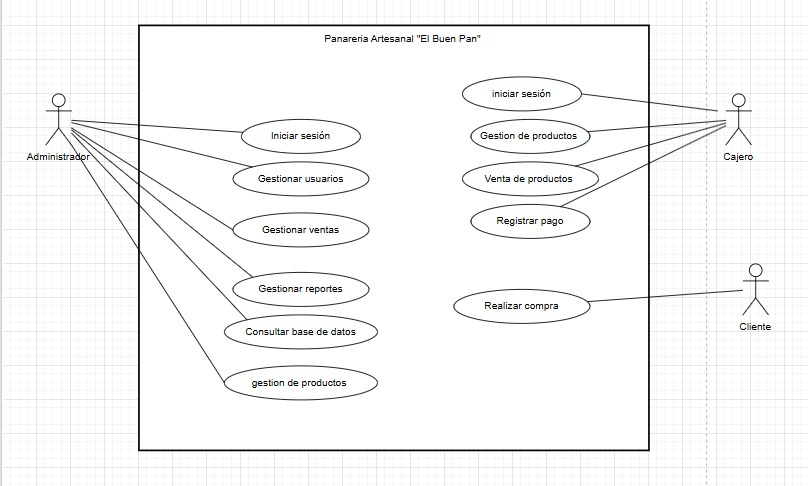
\includegraphics[width=0.9\columnwidth]{images/diagrama_casos_uso.jpg}}
\caption{Diagrama de Casos de Uso del Sistema de Gestión.}
\label{fig:casos_uso}
\end{figure}

\subsection{Diagrama de Clases}
Este diagrama representa la estructura estática del sistema. Modela las clases principales (Producto, Insumo, Venta, Usuario), sus atributos, métodos y las relaciones entre ellas (asociación, herencia, etc.), sirviendo como plano para la construcción de la base de datos y el backend.

%%% INSTRUCCIÓN: AQUÍ VA TU DIAGRAMA DE CLASES
%%% Guarda tu imagen como "diagrama_clases.png" en la misma carpeta y descomenta el código.
\begin{figure}[htbp]
\centerline{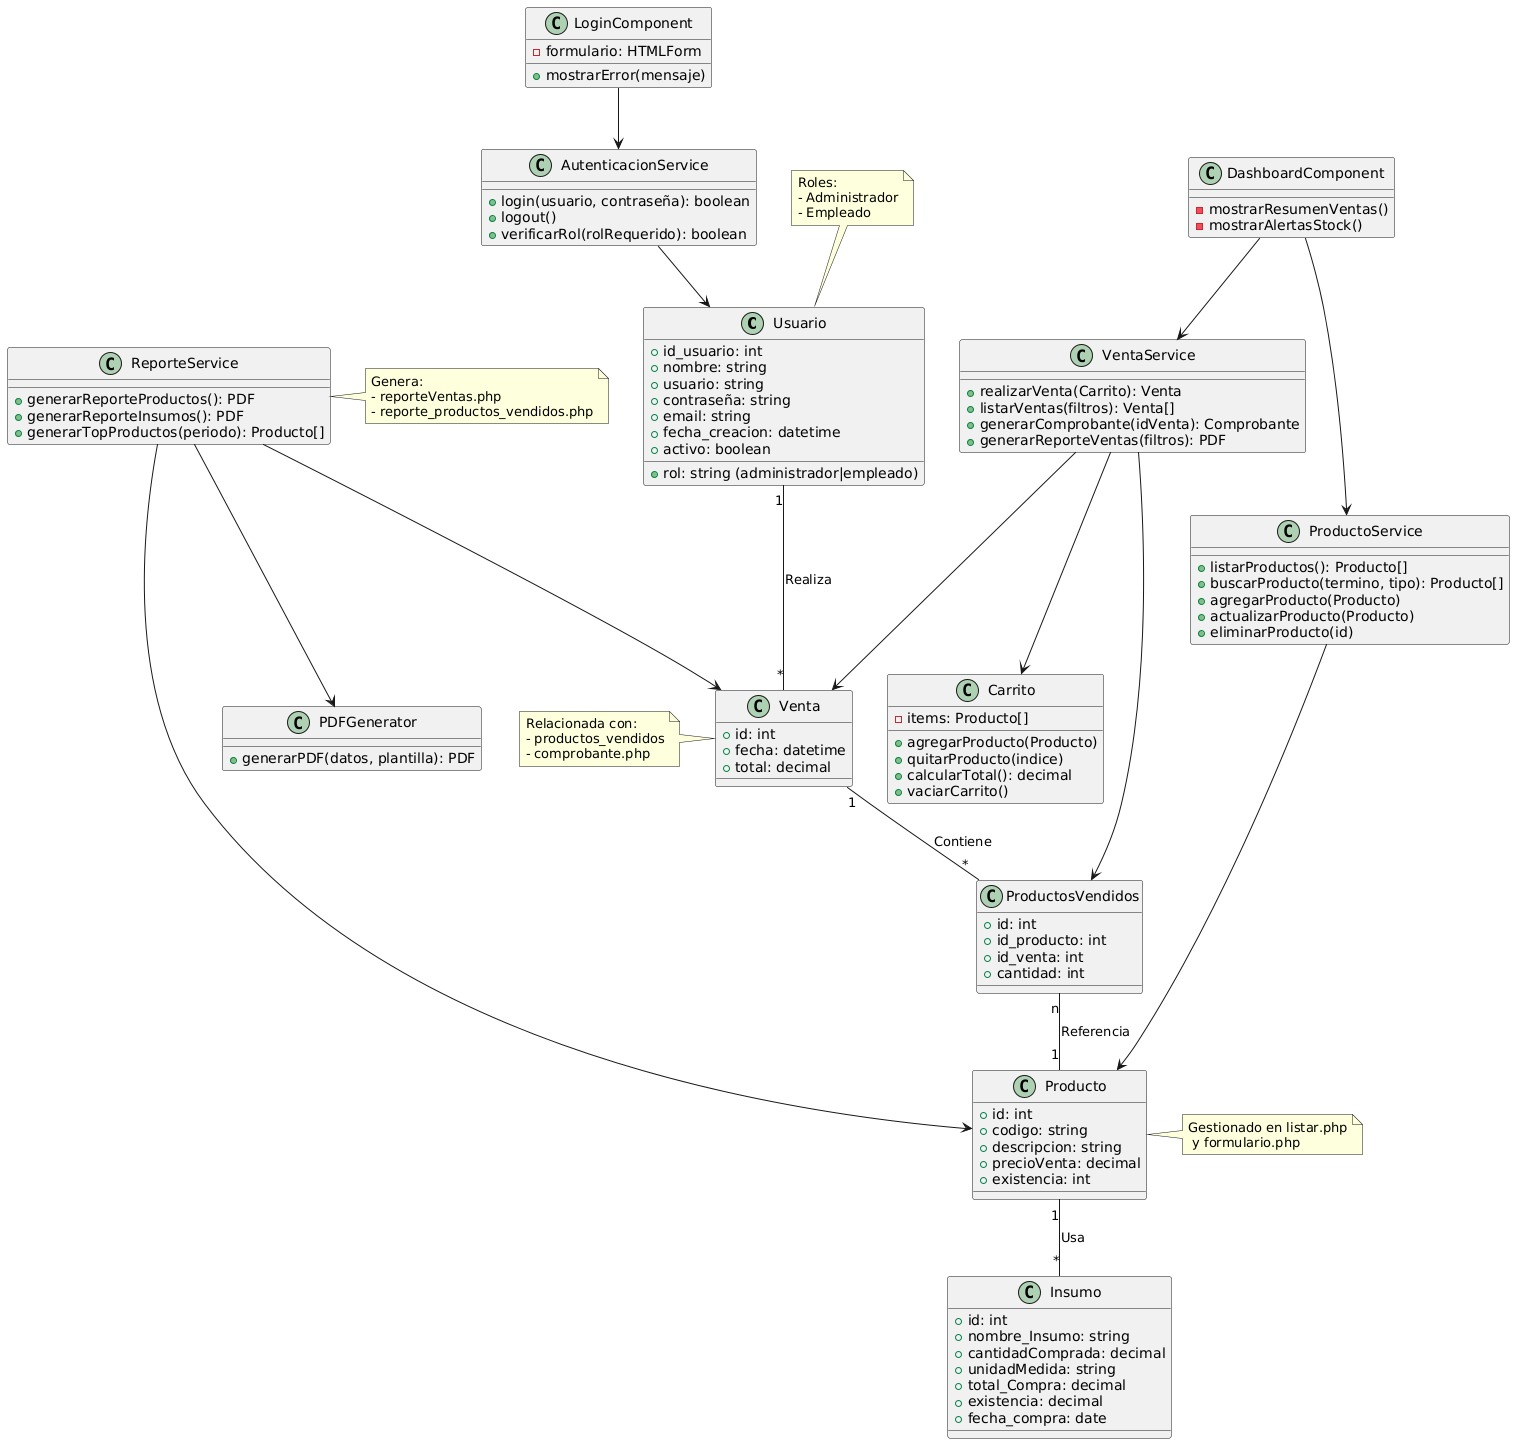
\includegraphics[width=\columnwidth]{images/diagrama_clases.jpg}}
\caption{Diagrama de Clases que modela la estructura del sistema.}
\label{fig:clases}
\end{figure}


\section{Metodología de Desarrollo}
\subsection{Metodología Utilizada}

Se adoptó Scrum como metodología ágil para el desarrollo del sistema de información de la panadería "El Buen Pan". Scrum fue elegido por su capacidad de adaptación a cambios, colaboración efectiva y entrega iterativa de funcionalidades.

\subsection{Roles en SCRUM}
\begin{itemize}
    \item \textbf{Product Owner:} Representante del cliente y responsable de gestionar el backlog del producto, priorizando requisitos y asegurando el valor del negocio.
    \item \textbf{Scrum Master:} Facilitador del equipo, responsable de eliminar obstáculos, promover un ambiente colaborativo y asegurar el cumplimiento de los principios y prácticas de Scrum.
    \item \textbf{Equipo de Desarrollo:} Equipo multidisciplinario responsable de diseñar, desarrollar, probar e implementar las funcionalidades del sistema.
\end{itemize}

%%% ====================================================================
%%% LUGAR PARA DIAGRAMA DE ACTIVIDADES
%%% ====================================================================
\subsection{Diagrama de Actividades del Proceso Scrum}
El flujo de trabajo del proyecto siguió el ciclo de vida de Scrum. El siguiente diagrama de actividades ilustra el flujo desde la planificación del sprint, pasando por las reuniones diarias, hasta la revisión y retrospectiva, mostrando el carácter iterativo del proceso.

%%% INSTRUCCIÓN: AQUÍ VA TU DIAGRAMA DE ACTIVIDADES
%%% Guarda tu imagen como "diagrama_actividades.png" en la misma carpeta y descomenta el código.
\begin{figure}[htbp]
\centerline{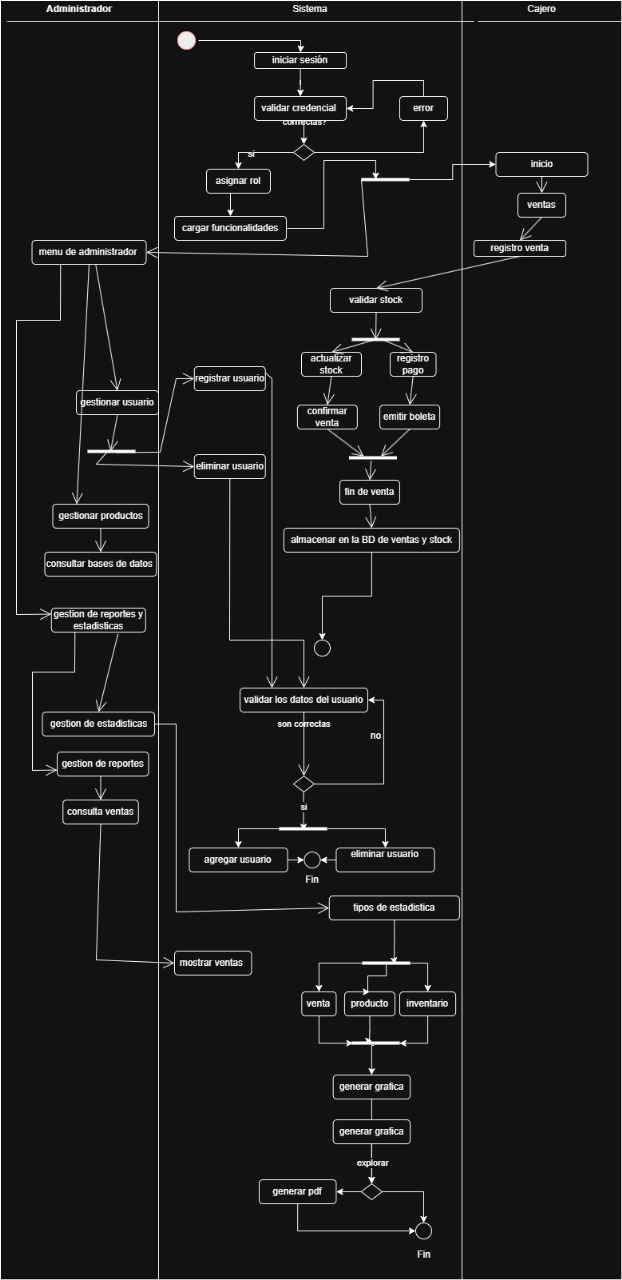
\includegraphics[width=0.9\columnwidth]{images/diagrama_actividades.jpg}}
\caption{Diagrama de Actividades del ciclo de desarrollo con Scrum.}
\label{fig:actividades}
\end{figure}

\subsection{Ceremonias de Scrum}
\subsubsection{Sprint Planning (Planificación del Sprint)} Al inicio de cada sprint de 2 semanas, el equipo realiza una reunión para seleccionar los elementos del backlog que se abordarán y establecer el objetivo del sprint.

\subsubsection{Daily Scrum (Reunión Diaria)} Reunión diaria de 15 minutos donde el equipo comparte el progreso, identifica obstáculos y ajusta el plan para cumplir con el objetivo del sprint.

\subsubsection{Sprint Review (Revisión de Sprint)} Al finalizar cada sprint, el equipo demuestra las funcionalidades completadas al Product Owner y otros stakeholders para obtener retroalimentación y ajustar el backlog.

\subsubsection{Sprint Retrospective (Retrospectiva de Sprint)} Reunión al final de cada sprint donde el equipo reflexiona sobre sus procesos de trabajo, identifica mejoras y define acciones para implementar en el próximo sprint.

\subsection{Proceso de Desarrollo}
El proceso se dividió en los siguientes sprints:
\begin{itemize}
    \item \textbf{Sprint 1: Requerimientos y Diseño Inicial} El equipo se reúne con el cliente para capturar y priorizar los requisitos. Se creó el backlog inicial y se establecieron los criterios de aceptación. Se realizó un diseño arquitectónico de alto nivel.
    \item \textbf{Sprint 2: Implementación Inicial} El equipo comenzó la implementación de las funcionalidades prioritarias. Se realizaron pruebas unitarias y de integración.
    \item \textbf{Sprint 3: Iteración y Refinamiento} Se continuó con el desarrollo de nuevas funcionalidades y se refinaron las existentes según las retroalimentaciones. Se aplicaron pruebas funcionales.
    \item \textbf{Sprint 4: Finalización de Funcionalidades} El equipo completó las funcionalidades restantes. Se enfocaron en la estabilización y optimización.
    \item \textbf{Sprint 5: Pruebas Finales y Puesta en Marcha} Se llevaron a cabo pruebas de aceptación con usuarios finales. Se preparó la documentación y se realizó el despliegue.
    \item \textbf{Post-Sprint: Soporte y Mantenimiento} Después del despliegue, se proporcionó soporte continuo y se realizó una retrospectiva final.
\end{itemize}

\section{Cronograma de Actividades}
\subsection{Sprint 1: Requerimientos y Diseño (Semanas 1-2)}
\begin{itemize}
    \item Captura y priorización de requisitos.
    \item Creación del backlog inicial del producto.
    \item Establecimiento de criterios de aceptación.
\end{itemize}

\subsection{Sprint 2: Implementación Inicial (Semanas 3-4)}
\begin{itemize}
    \item Desarrollo de funcionalidades prioritarias.
    \item Realización de pruebas unitarias y de integración.
\end{itemize}

\subsection{Sprint 3: Iteración y Refinamiento (Semanas 5-6)}
\begin{itemize}
    \item Desarrollo continuo y refinamiento de funcionalidades.
    \item Aplicación de pruebas funcionales y corrección de errores.
\end{itemize}

\subsection{Sprint 4: Finalización (Semanas 7-8)}
\begin{itemize}
    \item Completado de funcionalidades restantes.
    \item Estabilización del sistema y optimización.
\end{itemize}

\subsection{Sprint 5: Pruebas y Despliegue (Semanas 9-10)}
\begin{itemize}
    \item Pruebas de aceptación con usuarios finales.
    \item Preparación de documentación y despliegue.
\end{itemize}

\subsection{Post-Sprint: Soporte (Semana 11 en adelante)}
\begin{itemize}
    \item Soporte continuo a usuarios finales.
    \item Realización de retrospectiva final del proyecto.
\end{itemize}

\section{Descripción del Sistema de Información}
\subsection{Arquitectura del Sistema}
\begin{itemize}
    \item \textbf{Frontend:} Se utilizó React para el desarrollo de la interfaz de usuario, proporcionando una experiencia interactiva y fluida.
    \item \textbf{Backend:} Se implementó utilizando Node.js y Express, lo que permite una gestión eficiente de las solicitudes.
    \item \textbf{Base de Datos:} Se utilizó MongoDB como base de datos NoSQL, para una gestión flexible y escalable.
    \item \textbf{Servidor y Entorno:} Se desplegó en un servidor cloud y se utilizó Docker para contenerizar la aplicación.
\end{itemize}

%%% ====================================================================
%%% LUGAR PARA DIAGRAMA DE FLUJO
%%% ====================================================================
\subsection{Diagrama de Flujo del Proceso de Venta}
Para ilustrar una funcionalidad clave, el siguiente diagrama de flujo detalla los pasos del proceso de una venta en el sistema, desde que el vendedor inicia la transacción hasta que se actualiza el inventario y se genera el comprobante.

%%% INSTRUCCIÓN: AQUÍ VA TU DIAGRAMA DE FLUJO
%%% Guarda tu imagen como "diagrama_flujo.png" en la misma carpeta y descomenta el código.
\subsection{Diagrama de Flujo del Proceso de Venta}
Para ilustrar una funcionalidad clave, el siguiente diagrama de flujo detalla los pasos del proceso de una venta en el sistema, desde que el vendedor inicia la transacción hasta que se actualiza el inventario y se genera el comprobante.

\begin{figure}[htbp]
\centering
\begin{tikzpicture}[
    % Opciones de escalado para que el diagrama encaje
    scale=0.8, transform shape,
    node distance=1.3cm and 1.5cm,
    % Estilos de los bloques
    startstop/.style = {rounded rectangle, minimum width=3cm, minimum height=1cm, text centered, draw=black, fill=gray!20},
    process/.style   = {rectangle, minimum width=3cm, minimum height=1cm, text centered, text width=3.5cm, draw=black, fill=orange!30},
    decision/.style  = {diamond, aspect=1.8, minimum width=3cm, minimum height=1cm, text centered, draw=black, fill=cyan!30},
    io/.style        = {trapezium, trapezium left angle=70, trapezium right angle=110, minimum width=3cm, minimum height=1cm, text centered, text width=3cm, draw=black, fill=green!30},
    arrow/.style     = {thick, -{Stealth[length=3mm, width=2mm]}}
]
    % --- Posicionamiento de los nodos del diagrama ---
    \node (start) [startstop] {Inicio};
    \node (proc1) [process, below=of start] {Vendedor inicia nueva transacción en el sistema};
    \node (proc2) [process, below=of proc1] {Seleccionar productos y especificar cantidad};
    \node (dec1) [decision, below=of proc2, yshift=-0.5cm] {¿Confirmar Venta?};
    
    % Rama del "Sí"
    \node (proc3) [process, below=of dec1, yshift=-0.8cm] {Registrar venta en la Base de Datos};
    \node (proc4) [process, below=of proc3] {Actualizar inventario (reducir stock)};
    \node (io1) [io, below=of proc4] {Generar e mostrar comprobante de venta};
    \node (stop) [startstop, below=of io1] {Fin};
    
    % Rama del "No"
    \node (proc_cancel) [process, right=of dec1, xshift=0.5cm] {Cancelar transacción y volver al inicio};

    % --- DIBUJO DE CONEXIONES USANDO \draw ---
    \draw [arrow] (start) -- (proc1);
    \draw [arrow] (proc1) -- (proc2);
    \draw [arrow] (proc2) -- (dec1);
    
    % Conexiones de la rama "Sí"
    \draw [arrow] (dec1) -- node[anchor=east, pos=0.4] {Sí} (proc3);
    \draw [arrow] (proc3) -- (proc4);
    \draw [arrow] (proc4) -- (io1);
    \draw [arrow] (io1) -- (stop);
    
    % Conexiones de la rama "No" (CORREGIDO LÓGICA Y VISUALMENTE)
    \draw [arrow] (dec1) -- node[anchor=south, pos=0.2] {No} (proc_cancel);
    % La flecha ahora regresa al INICIO, como debe ser
    \draw [arrow] (proc_cancel.east) -- ++(1,0) |- (start);
    
\end{tikzpicture}
\caption{Diagrama de Flujo del módulo de ventas.}
\label{fig:flujo}
\end{figure}
\subsection{Funcionalidades Principales}
\begin{itemize}
    \item \textbf{Gestión de Insumos y Productos:} Permite el registro detallado de insumos comprados y la gestión de productos terminados (existencia, precios).
    \item \textbf{Registro y Gestión de Ventas:} Facilita el registro de ventas con detalles como fecha, productos, cantidad y precio total, permitiendo la generación de facturas.
    \item \textbf{Generación de Reportes:} Ofrece herramientas para generar reportes detallados sobre ventas, inventario y rentabilidad, exportables a PDF.
\end{itemize}

\subsection{Tecnologías Utilizadas}
\begin{itemize}
    \item \textbf{Frontend:} HTML5, CSS3, JavaScript (React), Bootstrap.
    \item \textbf{Backend:} Node.js, Express.
    \item \textbf{Base de Datos:} MySQL 8.0, MongoDB.
    \item \textbf{Control de Versiones:} Git y GitHub.
    \item \textbf{Despliegue:} Docker 4.43.2.
\end{itemize}

\section{Resultados y Evaluación}
\subsection{Logros Alcanzados}
\begin{itemize}
    \item \textbf{Automatización de Procesos Clave:} La automatización de la gestión de inventarios ha optimizado la precisión y eficiencia en el control de existencias.
    \item \textbf{Desarrollo de Interfaz de Usuario Intuitiva:} La interfaz diseñada proporciona una navegación amigable, aumentando la satisfacción de los usuarios.
    %%% INFORMACIÓN AÑADIDA
    \item \textbf{Disponibilidad de Datos para Decisión:} El sistema provee reportes en tiempo real, permitiendo al administrador tomar decisiones informadas sobre compras, producción y estrategias de venta.
\end{itemize}

\subsection{Evaluación del Sistema}
\begin{itemize}
    \item \textbf{Reducción del Tiempo de Gestión:} El sistema ha cumplido con los objetivos al mejorar la gestión operativa y aumentar la eficiencia.
    \item \textbf{Impacto en los Usuarios:} Se ha observado un impacto positivo en la satisfacción de los usuarios, quienes reportan una experiencia más fluida.
    \item \textbf{Eficiencia Operativa:} La implementación ha mejorado significativamente la eficiencia del negocio, reduciendo tiempos y optimizando recursos.
    \item \textbf{Perspectivas de Futuro:} Las funcionalidades implementadas sientan una base sólida para futuras expansiones y mejoras.
\end{itemize}

\section{Cuestionario de Evaluación (ISO 25010)}
A continuación se presenta el cuestionario utilizado para la evaluación de la calidad del software por parte de los usuarios finales.
\section{Cuestionario de Evaluación (Basado en ISO 25010)}
A continuación se presenta el cuestionario utilizado para la evaluación de la calidad del software por parte de los usuarios finales, basado en las características de la norma ISO 25010.

\begin{enumerate}
    \item \textbf{¿El sistema permite realizar todas las tareas necesarias para tu trabajo?}
        \begin{itemize}
            \item Muy en desacuerdo
            \item En desacuerdo
            \item Neutral
            \item De acuerdo
            \item Muy de acuerdo
        \end{itemize}

    \item \textbf{¿Los resultados generados por el sistema son correctos y confiables?}
        \begin{itemize}
            \item Muy en desacuerdo
            \item En desacuerdo
            \item Neutral
            \item De acuerdo
            \item Muy de acuerdo
        \end{itemize}
        
    \item \textbf{¿El sistema es fácil de aprender a usar?}
        \begin{itemize}
            \item Muy en desacuerdo
            \item En desacuerdo
            \item Neutral
            \item De acuerdo
            \item Muy de acuerdo
        \end{itemize}
        
    \item \textbf{¿La interfaz es clara y fácil de entender?}
        \begin{itemize}
            \item Muy en desacuerdo
            \item En desacuerdo
            \item Neutral
            \item De acuerdo
            \item Muy de acuerdo
        \end{itemize}
        
    \item \textbf{¿Te resulta cómodo realizar tus tareas en el sistema?}
        \begin{itemize}
            \item Muy en desacuerdo
            \item En desacuerdo
            \item Neutral
            \item De acuerdo
            \item Muy de acuerdo
        \end{itemize}
        
    \item \textbf{¿El sistema responde rápidamente a tus acciones?}
        \begin{itemize}
            \item Muy en desacuerdo
            \item En desacuerdo
            \item Neutral
            \item De acuerdo
            \item Muy de acuerdo
        \end{itemize}
        
    \item \textbf{¿Pudiste trabajar sin que el sistema se volviera lento?}
        \begin{itemize}
            \item Muy en desacuerdo
            \item En desacuerdo
            \item Neutral
            \item De acuerdo
            \item Muy de acuerdo
        \end{itemize}
        
    \item \textbf{¿El sistema funcionó sin errores o caídas durante el uso?}
        \begin{itemize}
            \item Muy en desacuerdo
            \item En desacuerdo
            \item Neutral
            \item De acuerdo
            \item Muy de acuerdo
        \end{itemize}
        
    \item \textbf{¿Sientes que puedes confiar en el sistema para tus tareas importantes?}
        \begin{itemize}
            \item Muy en desacuerdo
            \item En desacuerdo
            \item Neutral
            \item De acuerdo
            \item Muy de acuerdo
        \end{itemize}
        
    \item \textbf{¿Sientes que tu información está protegida al usar el sistema?}
        \begin{itemize}
            \item Muy en desacuerdo
            \item En desacuerdo
            \item Neutral
            \item De acuerdo
            \item Muy de acuerdo
        \end{itemize}
        
    \item \textbf{¿El sistema te solicita autenticación (usuario/contraseña) de forma segura?}
        \begin{itemize}
            \item Muy en desacuerdo
            \item En desacuerdo
            \item Neutral
            \item De acuerdo
            \item Muy de acuerdo
        \end{itemize}
        
    \item \textbf{¿Pudiste usar el sistema sin problema desde tu dispositivo o navegador?}
        \begin{itemize}
            \item Muy en desacuerdo
            \item En desacuerdo
            \item Neutral
            \item De acuerdo
            \item Muy de acuerdo
        \end{itemize}
        
    \item \textbf{¿Crees que el sistema sería fácil de actualizar o mejorar si fuera necesario?}
        \begin{itemize}
            \item Muy en desacuerdo
            \item En desacuerdo
            \item Neutral
            \item De acuerdo
            \item Muy de acuerdo
        \end{itemize}
        
    \item \textbf{¿Crees que este sistema podría usarse fácilmente en otros entornos?}
        \begin{itemize}
            \item Muy en desacuerdo
            \item En desacuerdo
            \item Neutral
            \item De acuerdo
            \item Muy de acuerdo
        \end{itemize}
        
    \item \textbf{¿Crees que el sistema cubre todas las funciones que su negocio necesita para operar sin problemas?}
        \begin{itemize}
            \item Muy en desacuerdo
            \item En desacuerdo
            \item Neutral
            \item De acuerdo
            \item Muy de acuerdo
        \end{itemize}
\end{enumerate}
Cada pregunta se evaluó en una escala de Likert de 1 (Muy en desacuerdo) a 5 (Muy de acuerdo).
%%% INFORMACIÓN AÑADIDA
\section{Conclusiones}
La implementación del sistema de gestión para la Panadería Artesanal "El Buen Pan" ha demostrado ser una solución efectiva para los desafíos operativos identificados. La automatización del inventario y las ventas no solo ha mejorado la eficiencia, sino que también ha proporcionado una base de datos robusta para el análisis de negocio. Los resultados de la evaluación de calidad del software indican una alta aceptación por parte de los usuarios, validando que el sistema es funcional, usable y fiable. El proyecto cumple exitosamente con el objetivo de optimizar los procesos clave de la panadería, sentando las bases para un crecimiento futuro sostenible.

% \begin{thebibliography}{00}
% \bibitem{b1} Su referencia aquí
% \end{thebibliography}

\end{document}